\documentclass[tikz,border=10pt]{standalone}
\usetikzlibrary{arrows.meta, positioning, shapes.geometric}

\begin{document}
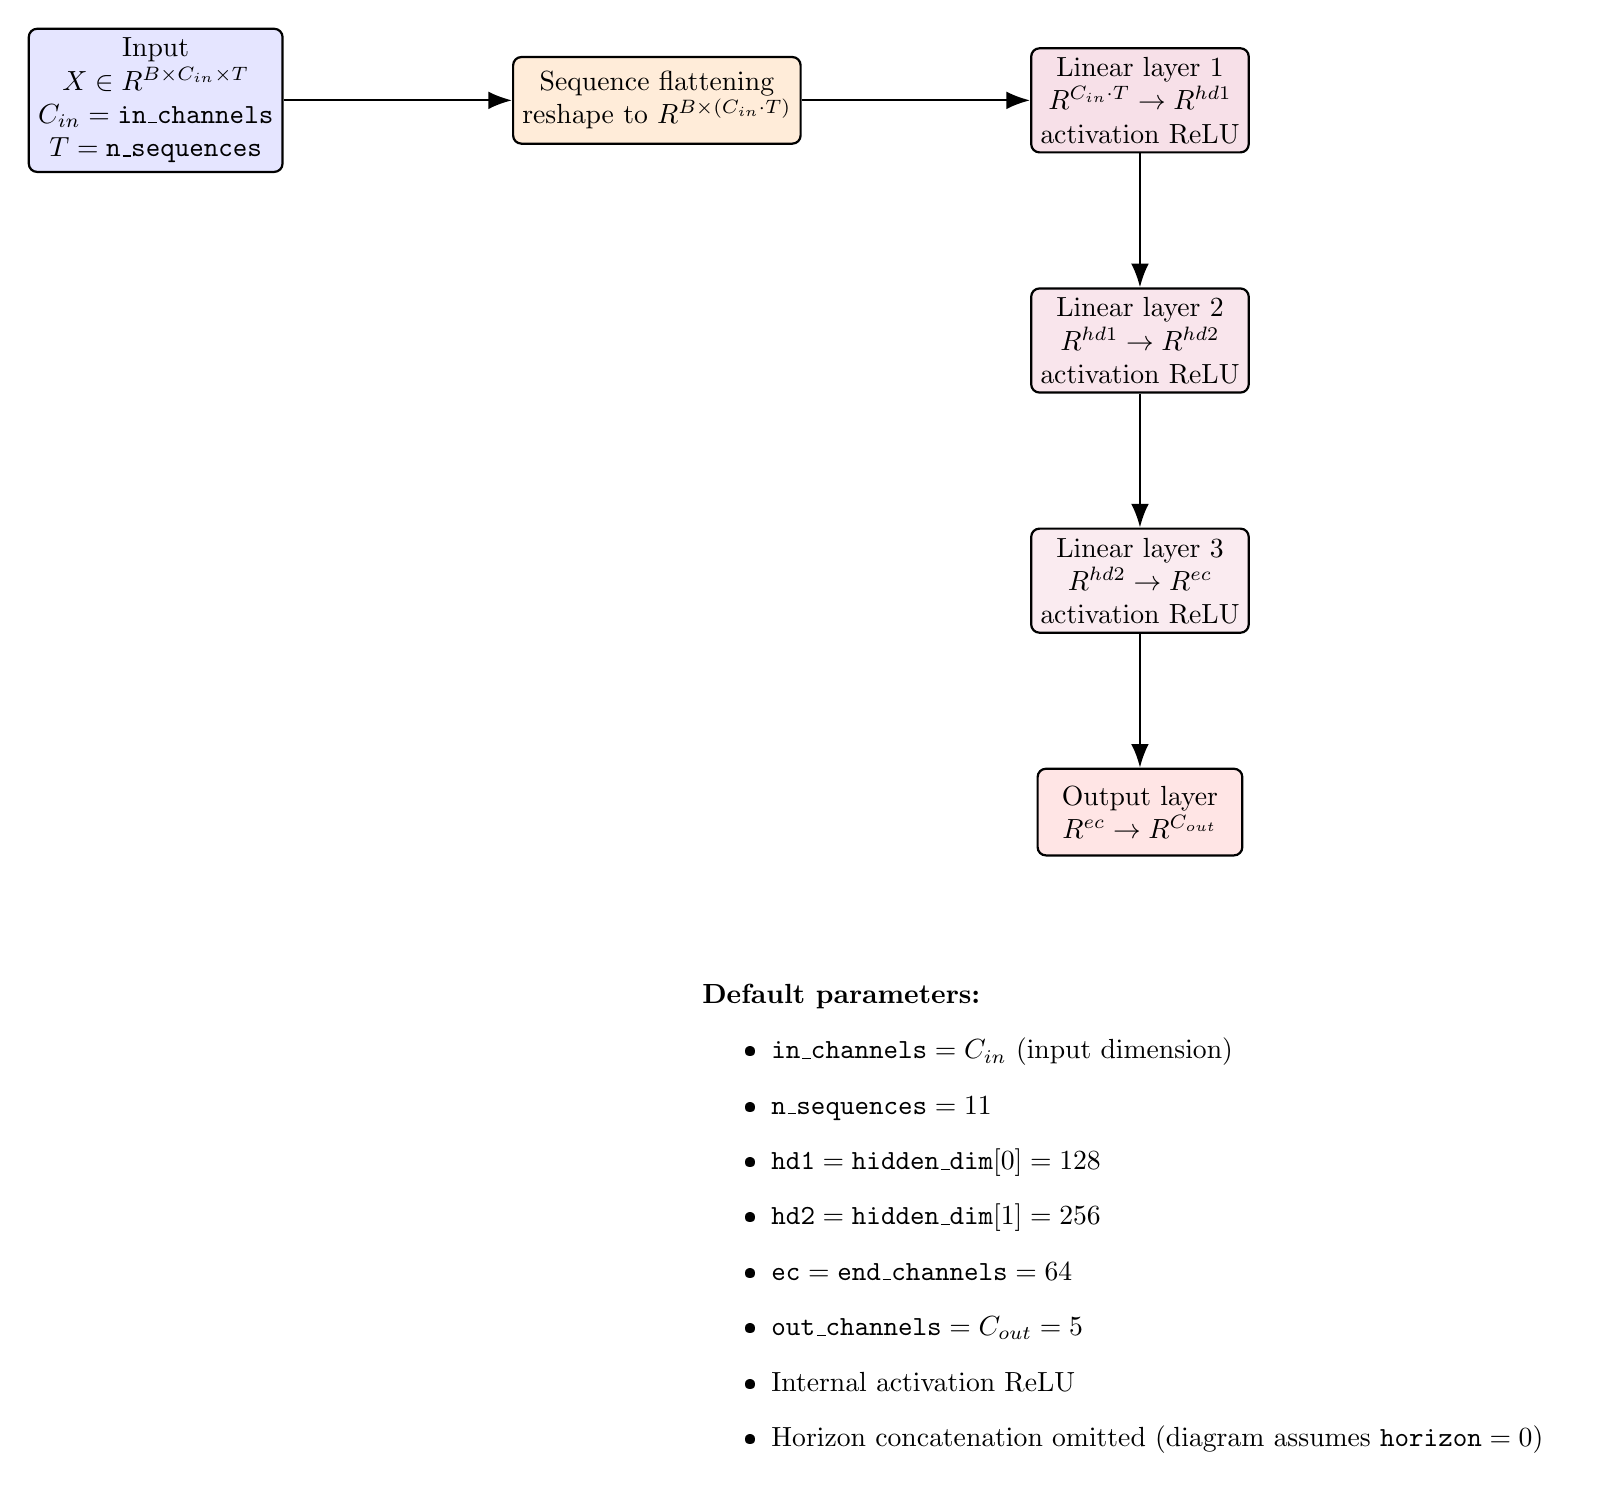
\begin{tikzpicture}[
    block/.style={draw, thick, minimum width=2.6cm, minimum height=1.1cm, align=center, rounded corners=3pt},
    arrow/.style={-{Latex[length=3mm]}, thick}
]
    % Input sequence information
    \node[block, fill=blue!10] (input) {Input\\$X \in \mathbb{R}^{B \times C_{in} \times T}$\\
        $C_{in} = \texttt{in\_channels}$\\
        $T = \texttt{n\_sequences}$};

    % Sequence flattening
    \node[block, right=2.9cm of input, fill=orange!15] (flatten) {Sequence flattening\\
        reshape to $\mathbb{R}^{B \times (C_{in} \cdot T)}$};

    \draw[arrow] (input) -- (flatten);

    % Linear layers and activations
    \node[block, right=2.9cm of flatten, fill=purple!12] (linear1) {Linear layer 1\\$\mathbb{R}^{C_{in} \cdot T} \rightarrow \mathbb{R}^{hd1}$\\
        activation ReLU};

    \draw[arrow] (flatten) -- (linear1);

    \node[block, below=1.7cm of linear1, fill=purple!10] (linear2) {Linear layer 2\\$\mathbb{R}^{hd1} \rightarrow \mathbb{R}^{hd2}$\\
        activation ReLU};

    \draw[arrow] (linear1) -- (linear2);

    \node[block, below=1.7cm of linear2, fill=purple!8] (linear3) {Linear layer 3\\$\mathbb{R}^{hd2} \rightarrow \mathbb{R}^{ec}$\\
        activation ReLU};

    \draw[arrow] (linear2) -- (linear3);

    \node[block, below=1.7cm of linear3, fill=red!10] (output) {Output layer\\$\mathbb{R}^{ec} \rightarrow \mathbb{R}^{C_{out}}$};

    \draw[arrow] (linear3) -- (output);

    % Legends for parameters
    \node[below=1.5cm of output, align=left] (legend) {
        \begin{minipage}{11cm}
            \textbf{Default parameters:}
            \begin{itemize}
                \item $\texttt{in\_channels} = C_{in}$ (input dimension)
                \item $\texttt{n\_sequences} = 11$
                \item $\texttt{hd1} = \texttt{hidden\_dim}[0] = 128$
                \item $\texttt{hd2} = \texttt{hidden\_dim}[1] = 256$
                \item $\texttt{ec} = \texttt{end\_channels} = 64$
                \item $\texttt{out\_channels} = C_{out} = 5$
                \item Internal activation ReLU
                \item Horizon concatenation omitted (diagram assumes $\texttt{horizon} = 0$)
            \end{itemize}
        \end{minipage}
    };

\end{tikzpicture}
\end{document}
